\section{Modello di sviluppo}
Il modello di sviluppo adottato dal gruppo è il \textbf{modello incrementale}.
\subsection{Modello incrementale}
Il modello di sviluppo incrementale vede il progetto come una serie di rilasci (interni e/o esterni), cosicché ad ogni scadenza il materiale consegnato sia sempre più vicino al prodotto finale.
Questo approccio di sviluppo vede la specifica del software, la sua implementazione, convalida ed evoluzione come attività intrecciate tra loro e da sviluppare in parallelo. Quindi il prodotto è considerato tale solo all'ultimo rilascio. Motivo per cui si relaziona bene con il versionamento adottato per il sistema.
L'adozione dello sviluppo incrementale porta i seguenti vantaggi:
\begin{itemize}
\item costi ridotti di implementazione;
\item facilità nell'ottenere feedback;
\item possibilità di consegnare prototipi.
\end{itemize}
Svantaggi del modello incrementale:
\begin{itemize}
\item il processo non è visibile e il manager deve richiedere consegne frequenti e regolari;
\item inclinazione alla degradazione del sistema, ovvero la difficoltà di aggiungere funzionalità al sistema in un rilascio successivo, dopo averne integrata un'altra nella consegna attuale. Ad ogni incremento aumenta la complessità del codice e di conseguenza dei costi. È possibile rimediare tramite refactoring, anche se quest'ultimo muta il modello di sviluppo da incrementale a iterativo.
\end{itemize}
\begin{figure}[H]
	\centering
	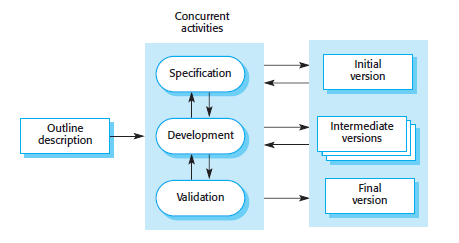
\includegraphics[width=0.70\linewidth]{img/incremental_development.png}
	\caption{Modello di sviluppo incrementale}
\end{figure}

\pagebreak
\subsubsection{Incrementi individuati}
Durante i periodi di Progettazione e Codifica per la Technology Baseline e Progettazione di Dettaglio sono stati individuati alcuni incrementi. \\
Di seguito verranno indicati tutti gli incrementi sviluppati con i relativi requisiti.

\begin{longtable}{C{4cm} L{3cm}}
\rowcolor{white}\caption{Tracciamento incrementi} \\
		\rowcolor{redafk}
\textcolor{white}{\textbf{Incremento}} &
\textcolor{white}{\textbf{Requisiti}} \\
		\endfirsthead
		\rowcolor{white}\caption[]{(continua)} \\
		\rowcolor{redafk}
\textcolor{white}{\textbf{Incremento}} &
\textcolor{white}{\textbf{Requisiti}} \\
		\endhead
Incremento 1: Sviluppo del tool di addestramento e conseguente ottenimento file JSON & Re1F1 \newline Re1F1.1  \newline Re1F1.2 \newline Re1F1.3 \newline Re2F1.6 \newline Re1F1.7 \newline Re1F13 \\
Incremento 2: Caricamento file JSON	nel plug-in & Re1F2 \newline Re1F2.1 \newline Re1F2.2  \newline Re1F2.4\\
Incremento 3: Collegamento plug-in al flusso dati & Re1F3.1 \newline Re1F3.2
\\
Incremento 4: Completamento tool di addestramento & Re1F1.4 \newline Re2F1.5 \newline Re1F11 \newline Re1F12
\\
Incremento 5: Completamento caricamento file JSON nel plugin & Re2F2.3
\\
Incremento 6: Collegamento del predittore al flusso dati e visualizzazione collegamenti & Re1F3.5 \newline Re1F4
\\
Incremento 7: Completamento pannello di collegamento & Re1F3 \newline Re1F3.4
\\
Incremento 8: Scollegamento dei predittori & Re1F5 \newline Re1F5.1 \newline Re1F5.2 \newline Re1F5.3 \newline Re2F5.4 \newline Re1F5.5 
\\
Incremento 9: \newline Modifica dei predittori & Re1F6 \newline Re1F6.1 \newline Re1F6.2 \newline Re1F6.3 \newline Re2F6.4 \newline Re1F6.5
\\
Incremento 10: Monitoraggio delle previsioni & Re1F7 \newline Re1F7.1 \newline Re2F7.2 \newline
\\
Incremento 11: Salvataggio previsioni sul database & Re1F8 \newline  Re1F8.1 \newline Re1F8.2 \newline Re1F8.3 \newline Re2F8.4 \newline Re1F8.5 \newline Re2F8.6
\\
Incremento 12: Visualizzazione dashboard previsioni  & Re1F10 \newline Re1F10.1
\\
Incremento 13: Interruzione monitoraggio & Re1F9 \newline Re1F9.1 \newline Re2F9.2
\\
Incremento 14: Inserimento messaggi di notifica/errori mancanti & Re1F14 \newline Re1F16 \newline Re1F17 \newline Re1F18
\\ 
\end{longtable}
\pagebreak
\subsection{Modello a componenti}
Per la realizzazione del prodotto sarà anche utilizzato, quando possibile, il modello di sviluppo a componenti, così da velocizzare e standardizzare lo
sviluppo dei requisti. I componenti evidenziati dall’analisi sono principalmente
gli elementi esistenti di Grafana e gli algoritmi di predizione (RL e SVM) forniti
da \textit{Zucchetti SPA}. In particolare tali elementi vengono inquadrati nelle seguenti classi di componenti: \begin{itemize}
\item \textbf{Grafana}: sono le librerie e le funzionalità fornite da Grafana, il loro uso viene quindi inquadrato come component reuse;
\item \textbf{Algoritmi di predizione}: sono gli algoritmi che ci sono stati forniti da \textit{Zucchetti SPA} e saranno riutilizzabili come librerie durante lo sviluppo del plug-in. Il loro uso viene quindi inquadrato come object and
function reuse.
\end{itemize}